\documentclass[]{elsarticle} %review=doublespace preprint=single 5p=2 column
%%% Begin My package additions %%%%%%%%%%%%%%%%%%%
\usepackage[hyphens]{url}

  \journal{Quaternary Science Reviews} % Sets Journal name


\usepackage{lineno} % add
  \linenumbers % turns line numbering on
\providecommand{\tightlist}{%
  \setlength{\itemsep}{0pt}\setlength{\parskip}{0pt}}

\usepackage{graphicx}
\usepackage{booktabs} % book-quality tables
%%%%%%%%%%%%%%%% end my additions to header

\usepackage[T1]{fontenc}
\usepackage{lmodern}
\usepackage{amssymb,amsmath}
\usepackage{ifxetex,ifluatex}
\usepackage{fixltx2e} % provides \textsubscript
% use upquote if available, for straight quotes in verbatim environments
\IfFileExists{upquote.sty}{\usepackage{upquote}}{}
\ifnum 0\ifxetex 1\fi\ifluatex 1\fi=0 % if pdftex
  \usepackage[utf8]{inputenc}
\else % if luatex or xelatex
  \usepackage{fontspec}
  \ifxetex
    \usepackage{xltxtra,xunicode}
  \fi
  \defaultfontfeatures{Mapping=tex-text,Scale=MatchLowercase}
  \newcommand{\euro}{€}
\fi
% use microtype if available
\IfFileExists{microtype.sty}{\usepackage{microtype}}{}
\bibliographystyle{elsarticle-harv}
\ifxetex
  \usepackage[setpagesize=false, % page size defined by xetex
              unicode=false, % unicode breaks when used with xetex
              xetex]{hyperref}
\else
  \usepackage[unicode=true]{hyperref}
\fi
\hypersetup{breaklinks=true,
            bookmarks=true,
            pdfauthor={},
            pdftitle={The Pleistocene-Holocene Transition in Tagua-Tagua, central Chile},
            colorlinks=false,
            urlcolor=blue,
            linkcolor=magenta,
            pdfborder={0 0 0}}
\urlstyle{same}  % don't use monospace font for urls

\setcounter{secnumdepth}{5}
% Pandoc toggle for numbering sections (defaults to be off)

% Pandoc citation processing
\newlength{\cslhangindent}
\setlength{\cslhangindent}{1.5em}
\newlength{\csllabelwidth}
\setlength{\csllabelwidth}{3em}
% for Pandoc 2.8 to 2.10.1
\newenvironment{cslreferences}%
  {}%
  {\par}
% For Pandoc 2.11+
\newenvironment{CSLReferences}[2] % #1 hanging-ident, #2 entry spacing
 {% don't indent paragraphs
  \setlength{\parindent}{0pt}
  % turn on hanging indent if param 1 is 1
  \ifodd #1 \everypar{\setlength{\hangindent}{\cslhangindent}}\ignorespaces\fi
  % set entry spacing
  \ifnum #2 > 0
  \setlength{\parskip}{#2\baselineskip}
  \fi
 }%
 {}
\usepackage{calc}
\newcommand{\CSLBlock}[1]{#1\hfill\break}
\newcommand{\CSLLeftMargin}[1]{\parbox[t]{\csllabelwidth}{#1}}
\newcommand{\CSLRightInline}[1]{\parbox[t]{\linewidth - \csllabelwidth}{#1}\break}
\newcommand{\CSLIndent}[1]{\hspace{\cslhangindent}#1}

% Pandoc header



\begin{document}
\begin{frontmatter}

  \title{The Pleistocene-Holocene Transition in Tagua-Tagua, central
Chile}
    \author[puc]{Matías Frugone-Álvarez\corref{1}}
   \ead{matutefrugone@gmail.com} 
    \author[uccs,ciba,geup]{Erwin Gonzáles Huerta}
  
    \author[ipe]{Blas Valero-Garcés}
  
    \author[uccs,ciba,geup]{Carolina Godoy}
  
    \author[uccs,ciba,geup]{Josu Aranbarri}
  
    \author[iact]{Penélope Gonzáles}
  
    \author[uccs,ciba,geup]{Antonio Delgado-Huerta}
  
    \author[deuc]{Claudio Latorre}
  
    \author[uccs,ciba,geup]{Rafael Labarca Encina}
  
      \address[puc]{Pontificia Universidad Católica de Chile,
Departamento de Ecología-Centro UC Desierto de Atacama, Av. Libertador
Bernardo O'Higgins 340, Santiago, Chile.}
    \address[ieb]{Instituto de Ecología y Biodiversidady (IEB),
Santiago, Chile}
    \address[uccs]{Instituto Pirenaico de Ecología (IPE-CSIC), Zaragoza,
Spain.}
    \address[ipe]{Centro de Investigación en Biodiversidad y Ambientes
Sustentables (CIBAS), Chile}
    \address[geup]{Department of Geology and Environmental Science,
University of Pittsburgh, Pittsburgh, USA}
    \address[iact]{Instituto Andaluz de Ciencias de la Tierra
(CSIC-UGR), Granada, Spain}
      \cortext[1]{Corresponding Author}
  
  \begin{abstract}
  Paleohydrological reconstructions from the Chilean Altiplano document
  abrupt moisture fluctuations during the last millennia. Although the
  end of the mid Holocene aridity and the onset of more humid conditions
  between 6--4 ka has been identified in numerous regional marine and
  terrestrial sites, the timing of late Holocene dry and humid phases
  shows large regional variability. Laguna Miscanti and Laguna Miñiques
  (23\(^\circ\) 43'S -- 67\(^\circ\) 46'W, 4140 m asl) are
  topographically closed, but connected by surface outflow from
  Miscanti. Sedimentological and geochemical indicators from two new
  cores show large facies changes, i.e.~higher carbonate and evaporite
  deposition during more arid periods and increased organic productivity
  (both algal and macrophyte) during more humid phases. As in most
  Andean lakes located in volcanic settings, large 14C reservoir effects
  occur complicating 14C dating, so the age models include 210Pb and
  U/Th dating. In spite of dating uncertainties, both lakes show similar
  patterns during the last millennium. A humid phase in Laguna Miscanti
  prior to ca 1200 CE is coherent with rodent middens and
  geomorphological features indicative of a major pluvial/recharge event
  at lower altitudes (Atacama Desert) during the Medieval Climate
  Anomaly (ca 800 - 1300 CE). The LIA (1300 -- 1850 CE) is characterized
  by several arid/humid cycles and the last century by a productivity
  increase. The hydrological changes observed during the last millennium
  illustrate the complex dynamics of recent climate evolution over the
  high altitude Andean plateau. Discrepancies between the northern and
  southern Altiplano records and with intermediate latitudes (Central
  Chile) records may reflect contrasting responses to external forcing
  (Westerlies versus South American Monsoon dynamics) along different
  climatic zones.
  \end{abstract}
   \begin{keyword} keywords\end{keyword}
 \end{frontmatter}

\hypertarget{introduction}{%
\section{Introduction}\label{introduction}}

\hypertarget{study-site-and-regional-setting}{%
\section{Study site and regional
setting}\label{study-site-and-regional-setting}}

\hypertarget{materials-and-methods}{%
\section{Materials and methods}\label{materials-and-methods}}

\hypertarget{sedimentary-and-geochemical-analysis}{%
\subsection{Sedimentary and geochemical
analysis}\label{sedimentary-and-geochemical-analysis}}

In November 2019, we recovered a sedimentary sequence
(\textasciitilde2.8 m) of the profile exposed on the western wall of the
geoarchaeological excavation Tagua-Tagua 3 in ALLT (Figure 1). Sediment
samples were obtained at 1-cm intervals and send at IPE-CSIC and
IACT-CSIC laboratories in Spain for the geochemical and isotopic
analyses. Subsamples were taken every 2 cm for analysed of total carbon
(TC), total inorganic carbon (TIC), total organic carbon
(\(TOC = T-TIC\)), total nitrogen (TN) and total sulfur (TS) in a LECO
SCN furnace (IPE--CSIC). The grain-size frequency distributions between
0.02 um and 2000 um were measured in triplicate using a Malvern
Mastersizer 2000 APA2000 grain-size analyzer with Hydro 2000G AWA2000.
The sample sto determiner the grain--size were pre-treated with 10\%
H2O2 and 10\% HCl to remove organic matter and carbonates, respectively.
Robust End-member mixing analysis (EMMA) analisis was performed using
the generic deterministic EMMA protocol (R package EMMAgeo, version:
0.9.8; Dietze et al 2012; Dietze and Dietze 2019) to infer the sediment
sources, transport and depositional processes.

IACT-CSIC (Granada)

Elemental geochemical every 1 cm for total carbon (TC), total inorganic
carbon (TIC), total organic carbon (\(TOC = T-TIC\)) and total sulfur
(TS) in a LECO SC 144 DR furnace (IPE--CSIC). Total nitrogen (TN) was
measured in a VARIO MAX CN elemental analyzer (IPE--CSIC). Grain--size
distributions between 0.02 um and 2000 um were measured using a Malvern
Mastersizer 2000 APA2000 grain-size analyzer with Hydro 2000G AWA2000.
Sedimentary facies were described based on criteria formulated by
(Schnurrenberger et al., 2003) and lacustrine units have been classified
according to the sedimentary structure, MSCL data, elemental composition
(TOC, TIC, TN, TS, TOC/TN, BioSi), XRF data and waxes composition.

\hypertarget{chronology}{%
\subsection{Chronology}\label{chronology}}

The radiocarbon sample on carbon and bulk sediment were obtained of the
profile exposed sampled at 1 cm resolution (Table 1) . The radiocarbon
ages were determined by AMS at DirectAMS laboratories, USA. Results are
presented in units of percent modern carbon (pMC) and the uncalibrated
radiocarbon age before present (BP).

\begin{center}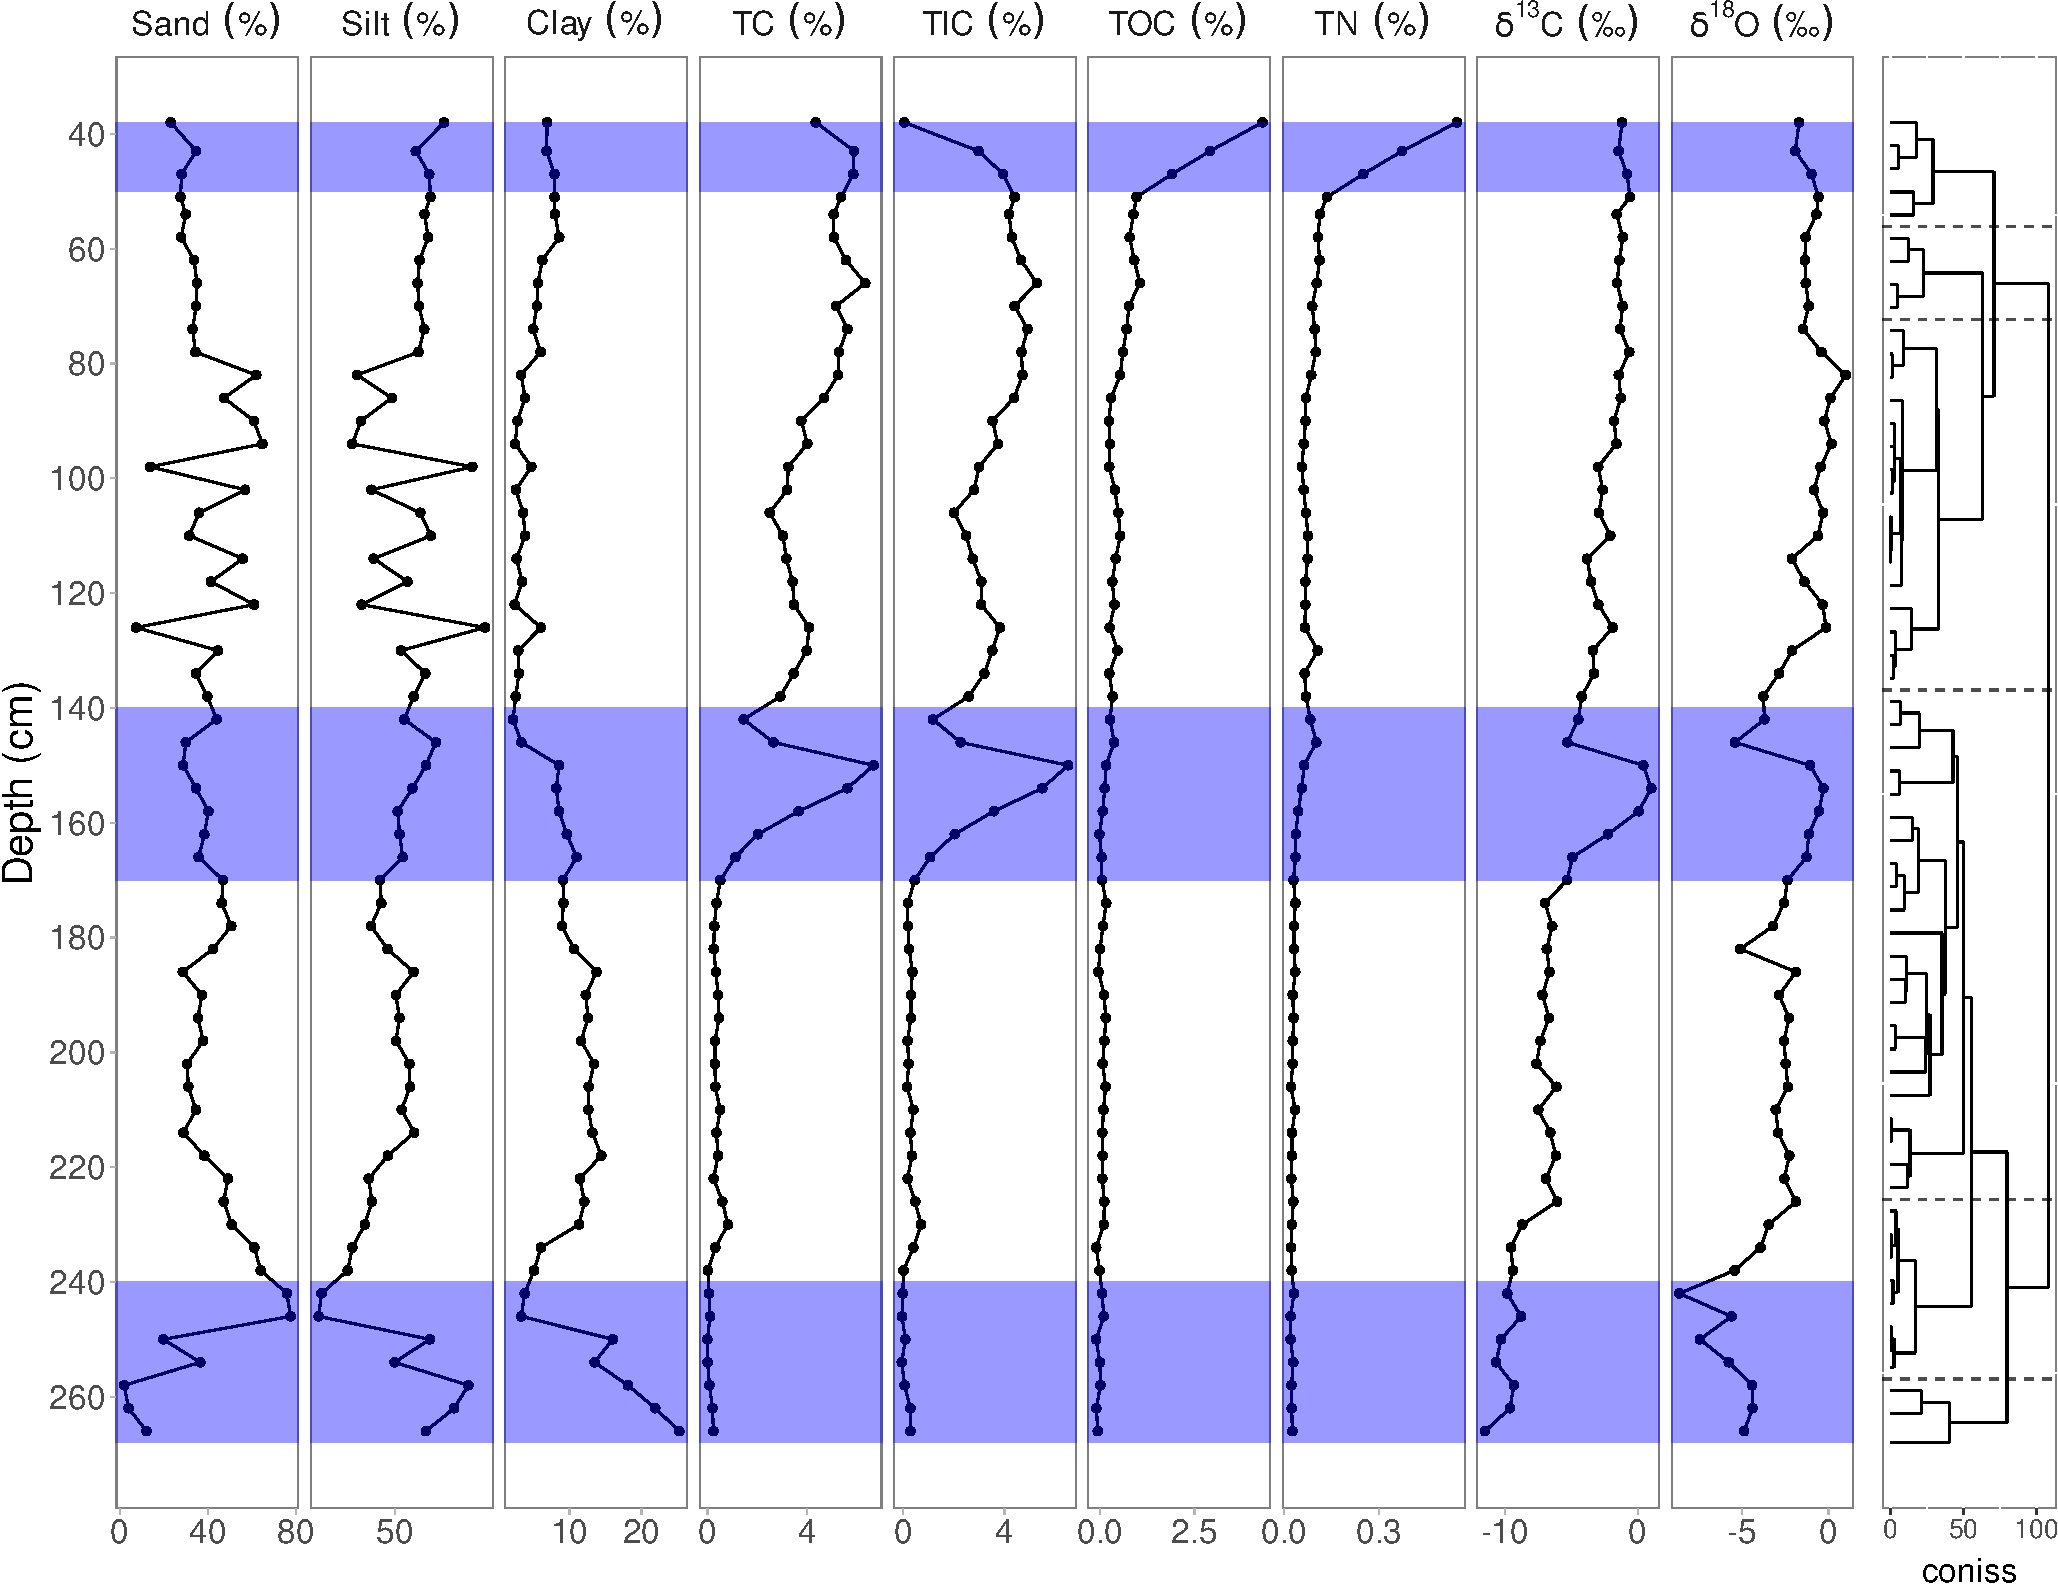
\includegraphics[width=1\linewidth]{paper_files/figure-latex/unnamed-chunk-2-1} \end{center}

\hypertarget{results}{%
\section{Results}\label{results}}

\hypertarget{cores-correlations-and-sedimentary-proxies}{%
\subsection{Cores correlations and sedimentary
proxies}\label{cores-correlations-and-sedimentary-proxies}}

\hypertarget{references}{%
\section*{References}\label{references}}
\addcontentsline{toc}{section}{References}

\hypertarget{refs}{}
\begin{CSLReferences}{1}{0}
\leavevmode\hypertarget{ref-schnurrenbergerClassificationLacustrineSediments2003}{}%
Schnurrenberger, D., Russell, J., Kelts, K., 2003. Classification of
lacustrine sediments based on sedimentary components. Journal of
Paleolimnology 29, 141--154.
doi:\href{https://doi.org/10.1023/A:1023270324800}{10.1023/A:1023270324800}

\end{CSLReferences}


\end{document}
